\chapter{Heuristics and Detection Algorithms}
    The gathered information about a process' behavior is used by heuristic algorithms to identify potentially malicious activity. As the name
    implies, these algorithms are not 100\% accurate and can result in false positives as well as false negatives. However, combining multiple
    heuristic detection algorithms has been proven to be an efficient detection technique.

    \section{Privilege Escalation Detection}
        Privilege escalation is a type of exploit that elevates a running process or starts an elevated process while bypassing operating system's
        security or user notification mechanisms (eg. User Account Control on Windows). In order to correctly identify the exploit it is essential
        to understand how elevation works on Windows. In this section I am going to go into detail about how Windows elevation works and the
        algorithm I used in order to detect it.

        \paragraph{}
        There are multiple legitimate ways of starting a process as admin:
        \begin{itemize}
            \item from an unprivileged process, via ShellExecuteEx % through UAC (User Account Control)
            \item request administrator rights at process start via manifest
            \item from a privileged process by simply calling CreateProcess
        \end{itemize}

        \paragraph{}
        However, there is no way to legitimately elevate an already running process.

        \paragraph{}
        In order for a process with no admin rights to start an elevated process, it has to send a request to svchost, which shows the User Account
        Control pop-up, notifying the user that the process needs admin rights. If admin rights are granted by UAC, svchost starts the process.
        This can be done with the ShellExecuteEx API, or by setting the requestedExecutionLevel field to "requireAdministrator" in the manifest
        file.

        Manifest snippet for requesting administrator rights on process start:
        \begin{verbatim}
<trustInfo xmlns="urn:schemas-microsoft-com:asm.v2">
<security>
<requestedPrivileges xmlns="urn:schemas-microsoft-com:asm.v3">
    <requestedExecutionLevel level="requireAdministrator" uiAccess="false" />
</requestedPrivileges>
</security>
</trustInfo>
        \end{verbatim}

        \paragraph{}
        If a process is already elevated, any process created by it will also be elevated by default. We can easily see that, if wsl.exe is
        started with admin rights, all Linux processes running in that WSL instance will be granted admin rights inside Windows, which would
        be disastrous considering the security of the computer.

        \paragraph{}
        An easy, yet not completely reliable method for detecting this type of exploit can be implemented in a kernel driver. A more reliable
        method would be using hypervisor memory introspection techniques, but I will only cover the first.

        \paragraph{}
        I'm going to describe the most basic way of detecting privilege escalation, which is, detecting if a process was maliciously started
        with admin rights. As I've previously mentioned, a process can start with admin rights if and only if its parent is elevated or it was started
        by a svchost. In order to do this, we need check whether or not the process is elevated in the process create callback. Below is a summary
        implementation for a function that takes a process handle and returns its current elevation status.

        \begin{Verbatim}[fontsize=\small, commandchars=\\\{\}]
ZwOpenProcessTokenEx(\textcolor{darkgray}{processHandle}, \textcolor{magenta}{GENERIC_READ}, \textcolor{magenta}{OBJ_KERNEL_HANDLE}, &token);
ZwQueryInformationToken(token, \textcolor{Apricot}{TokenElevation}, &tokenElevation,
                        \textcolor{blue}{sizeof}(tokenElevation), &returnLength);
\textcolor{blue}{return} tokenElevation.TokenIsElevated;
        \end{Verbatim}

        \paragraph{}
        Seeing how execve exploit works, it is clearly obvious that while this method works for the most basic case, it will not be enough for an
        exploit that elevates an already running process. Therefore, we need to check that the security token was not tampered with whenever we
        suspect that the process might be doing something potentially malicious. For example, any file operation done in the \%SystemRoot\%
        directory.

        At this point, it's easy to see several issues:

        \begin{itemize}
            \item if the exploit elevates a running process
            \item if the elevated process is a Windows process
            \item performance overhead added by polling the security token
        \end{itemize}

        Further, I will explain how I have tackled these issues and enhanced the algorithm.

        \paragraph{}
        In order to detect if a process was maliciously elevated after it was started, we need to keep track of monitored active processes in the
        called process collector, storing their initial elevation status. If the process was initially not elevated, it should never become
        elevated.

        Whenever a monitored process issues file operations for files in sensitive locations (i.e. C:\textbackslash Windows), we will recheck
        the security token with the described algorithm. If the new token query reveals that the process is elevated, and initially it was not,
        then the process should be detected and stopped.

        \pagebreak

        \begin{figure}[!ht]
            \centering
            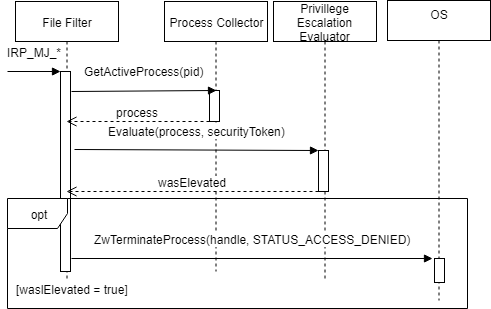
\includegraphics[width=310px,keepaspectratio]{img/privilege_escalation_detection_diagram.png}
            \caption{privilege escalation detection diagram}
            \label{fig:privilege_escalation_detection_diagram}
        \end{figure}

        
        A more detailed explanation for the diagram can be found below:

        \begin{enumerate}
            \item for any IRP filtered by the file filter we get the process from the collector
            \item we check if the process was elevated since it was started
            \item we kill the process if the process was elevated
        \end{enumerate}

        \paragraph{}
        Even though the vulnerability that led to the execve exploit\cite{execve} was fixed by Microsoft, we can see that the described algorithm
        is a generic approach as it does not take into consideration any particularities in the previously mention exploit.

    \section{File Infectors and Droppers Detection}
        \paragraph{}
        File infectors tamper with existing executables, injecting malicious code into them. Even though these can be prevented by the provider
        of the executable by digitally signing it, unsigned executables are vulnerable to being infected, posing a threat to the users that
        use them. Droppers however would write malicious executables on disk and are commonly disguised as installers or application bundles.

        \paragraph{}
        These are relatively simple to detect, as Linux processes would have no reason to create or modify Windows executables. The more
        complicated case is when a Linux process starts a Windows process to carry out the potentially malicious actions on behalf of the Linux
        process. Until now, there haven't been observed any WSL applications interact with Windows processes it is still not clear how to
        classify this behavior. For now, until the market evolves, the safer decision would be to treat Windows processes that are in a
        Linux process tree (there is at least a Linux process ancestor) same as Linux processes. This means that whether the Linux process
        drops an executable or starts a Windows process to drop it, both cases would cause a detection that kills the whole tree (up to the
        last Linux process).

        \paragraph{}
        The relevant action a file infector does writing in Windows executable files, which actually is a
        IRP\textunderscore MJ\textunderscore WRITE operation in terms of file system filtering.
